\section{Results and Discussion}\label{sec:results}

This section reports preliminary results from the unified 9-hour training. All values come from the patient-level holdout (\nTest{} images/\nTestPatients{} patients) or an explicitly labelled clean-official subset; train-self is never presented as generalisation. Because the budget is a single holdout rather than five-fold and several models are not fully converged, we frame the results as reproducible preliminary evidence, not as a claim of optimality.

\subsection{Main Patient-Level Results}

Table~\ref{tab:main-gland} reports gland segmentation on the patient-level test set. All models use the same preprocessing, split, loss, and 384 tile; MGD-Former uses an ADE20K-pretrained encoder, while the others are randomly initialised. Means, 95\% bootstrap confidence intervals, and valid $n$ are reported.

\begin{table}[t]
\centering
\caption{Gland segmentation on the patient-level test set (mean; 95\% bootstrap CI in parentheses; $n=\nTest$).}
\label{tab:main-gland}
\small
\resizebox{\linewidth}{!}{%
\begin{tabular}{lcccccc}
\toprule
Model & Dice & IoU & clDice & HD95 (px) & ASSD (px) & Params \\
\midrule
MGD-Former & \gDiceMF & \gIoUMF & \gClDiceMF & \gHDMF & \gASSDMF & $\sim$27M \\
UNet & \gDiceUNet & \gIoUUNet & \gClDiceUNet & \gHDUNet & \gASSDUNet & 31.2M \\
AttentionUNet & \gDiceAtt & \gIoUAtt & \gClDiceAtt & \gHDAtt & \gASSDAlt & $\sim$34M \\
MGD-PriorNet & \gDicePrior & \gIoUPrior & \gClDicePrior & \gHDPrior & \gASSDPrior & 1.5M \\
\bottomrule
\end{tabular}}
\end{table}

Three observations follow. First, absolute Dice under a patient-level split is lower than image-level literature values; this is expected, because images of the same subject no longer cross training and test, and the model must generalise to new patients. Second, MGD-Former and AttentionUNet reach \gDiceMF{} and \gDiceAtt{} respectively, within 0.01 of each other; we therefore do not declare an architectural winner, but treat them as comparable and inspect clDice/HD95 for topological differences. MGD-Former's ADE20K pretraining did not provide the large advantage often assumed, which contrasts with the common ``pretraining solves cold start'' narrative. Third, UNet's \gDiceUNet{} is clearly lower, showing that 30 epochs from scratch are insufficient here; however, its clDice is the highest (\gClDiceUNet{} vs \gClDiceMF{}), indicating that clDice is insensitive to over-segmentation/width and cannot be used alone for ranking. MGD-PriorNet reaches \gDicePrior{} at 1.5M parameters with paired Wilcoxon $p=\pMFPrior$, not significantly different from MGD-Former, suggesting that anatomical priors can be more cost-effective in a tiny model. These comparisons are confounded by epoch budget and pretraining, and must not be read as an architecture ranking.

Two boundaries must be explicit. First, \textbf{MGD-Former uses ADE20K pretraining while the other models are randomly initialised}; the main-table gap includes the pretraining benefit and cannot be attributed to architecture alone. The 9-hour budget did not include a random-init MGD-Former control; this is a limitation and a target for the five-fold extension. Second, \textbf{WRCANet is excluded from the main ranking}: it needs about 38\,min per epoch on the 8\,GB card and completed only one epoch (val Dice 0.006) within budget, so it is not converged; this demonstrates memory/time feasibility, not architectural quality. AttentionUNet was continued to 15 epochs and MGD-PriorNet reached about 12; neither is fully converged, so their values should be read as such.

Paired Wilcoxon tests on the same patient-level test set (per-sample Dice): MGD-Former vs AttentionUNet $p=\pMFAtt$, vs UNet $p=\pMFUNet$, vs MGD-PriorNet $p=\pMFPrior$. Statistical significance is not clinical importance: if the mean difference between AttentionUNet and MGD-Former is within 0.01, it should be reported as ``comparable'', not as a win; architecture ranking is not the main conclusion of this paper.

\subsection{The Cost of Leakage}

Table~\ref{tab:leakage} compares patient-level and image-level leaky UNets on the clean-official \cleanOfficialImages{} images/\cleanOfficialPatients{} patients. The two share architecture, loss, epoch budget, and inference protocol; the only difference is whether the training split contains other images of official-test patients.

\begin{table}[t]
\centering
\caption{Leakage control on the clean-official subset (UNet; $n=\cleanOfficialImages$).}
\label{tab:leakage}
\small
\begin{tabular}{lc}
\toprule
Protocol & Dice \\
\midrule
patient-level & \leakDiceClean \\
image-level leaky & \leakDiceLeaky \\
Difference (leaky $-$ clean) & \leakDelta \\
\bottomrule
\end{tabular}
\end{table}

\begin{figure}[t]
\centering
\ifnum\resultsavailable=1
\begin{tikzpicture}
\begin{axis}[
  width=0.72\linewidth, height=5.2cm,
  ybar, bar width=18pt,
  ymin=0, ymax=1,
  ylabel={Dice (clean-official)},
  symbolic x coords={Patient-level, Leaky},
  xtick=data,
  nodes near coords,
  nodes near coords style={font=\scriptsize},
  tick label style={font=\scriptsize},
  label style={font=\scriptsize},
  enlarge x limits=0.45,
  axis lines=left,
]
\addplot[fill=teal!65, draw=teal!80] coordinates {
  (Patient-level,\leakDiceClean)
  (Leaky,\leakDiceLeaky)
};
\end{axis}
\end{tikzpicture}
\else
\fbox{\parbox[c][4.5cm][c]{0.72\linewidth}{\centering\small Leakage results pending: clean-official \cleanOfficialImages{} images/\cleanOfficialPatients{} patients}}
\fi
\caption{Leakage cost on the official clean-official subset. Both bars use the same UNet, epoch budget, and inference protocol; only the training split differs. Difference $\Delta=\leakDelta$.}
\label{fig:leakage}
\end{figure}


In this budget the leaky control is actually lower: patient-level \leakDiceClean{} vs leaky \leakDiceLeaky{} ($\Delta=\leakDelta$), so no inflation was observed. There are three plausible reasons: the leaky model trained for only 20 epochs (patient-level UNet for 30), the official 200 has a different difficulty distribution, and clean-official contains only 60 images. The overlap statistics (326/800, 116/166) prove that the leakage risk is real, but performance inflation is not confirmed by this run; we report it as an audit, not as a conclusion.

\subsection{Tiling, MTE, and TTA}

Table~\ref{tab:tta} uses MGD-Former to compare the default 384 tile, MTE (probability average of 256/384/512), and 8$\times$ TTA. MTE requires no retraining and costs about 3$\times$ inference; 8$\times$ TTA costs about 8$\times$.

\begin{table}[t]
\centering
\caption{Tiling and TTA (MGD-Former; patient-level test set).}
\label{tab:tta}
\small
\begin{tabular}{lcccc}
\toprule
Protocol & Dice & clDice & HD95 (px) & Relative inference cost \\
\midrule
384 single tile & \gDiceMF & \gClDiceMF & \gHDMF & 1$\times$ \\
MTE (256/384/512) & \mteDiceMF & \mteClDiceMF & \mteHDMF & $\sim$3$\times$ \\
8$\times$ TTA & \ttaEight & \ph & \ph & $\sim$8$\times$ \\
\bottomrule
\end{tabular}
\end{table}

\begin{figure}[t]
\centering
\ifnum\resultsavailable=1
\begin{tikzpicture}
\begin{axis}[
  width=0.78\linewidth, height=5.2cm,
  ybar, bar width=16pt,
  ymin=0, ymax=1,
  ylabel={Dice},
  symbolic x coords={384 single, MTE, 8x TTA},
  xtick=data,
  nodes near coords,
  nodes near coords style={font=\scriptsize},
  tick label style={font=\scriptsize},
  label style={font=\scriptsize},
  enlarge x limits=0.25,
  axis lines=left,
  legend style={font=\scriptsize, at={(0.5,-0.22)}, anchor=north, legend columns=3},
]
\addplot[fill=slate!35, draw=slate!70] coordinates {(384 single,\gDiceMF)};
\addplot[fill=teal!65, draw=teal!80] coordinates {(MTE,\mteDiceMF)};
\addplot[fill=alert!45, draw=alert!70] coordinates {(8x TTA,\ttaEight)};
\legend{Single tile,MTE,8$\times$ TTA}
\end{axis}
\end{tikzpicture}
\else
\fbox{\parbox[c][4.5cm][c]{0.78\linewidth}{\centering\small MTE/TTA results pending: same MGD-Former weights, patient-level test set}}
\fi
\caption{Accuracy--cost trade-off of tiling and TTA. MTE averages 256/384/512 probabilities and costs about 3$\times$; 8$\times$ TTA costs about 8$\times$.}
\label{fig:mte}
\end{figure}


MTE did not beat 384 on Dice (\mteDiceMF{} vs \gDiceMF{}), but it reduced HD95 from \gHDMF{} to \mteHDMF{}, indicating that it mainly improves boundaries/outliers rather than pixel overlap; 8$\times$ TTA gives a small Dice gain (\ttaEight{}) at about 8$\times$ cost. MTE should therefore be positioned as a stable, low-cost boundary correction, not as a method that adds accuracy. Tiling sensitivity remains a strong finding, but ``changing the tile reliably adds Dice'' does not hold in this run.

\subsection{Uncertainty-Guided Review}

Table~\ref{tab:uncertainty} reports AUROC for three uncertainty signals on failure cases (Dice $<0.7$). Multi-tile variance $V$ is already available from MTE; entropy $H$ is almost free; 8$\times$ TTA is the most expensive.

\begin{table}[t]
\centering
\caption{AUROC for failure detection (MGD-Former; failure defined as Dice $<0.7$).}
\label{tab:uncertainty}
\small
\begin{tabular}{lccc}
\toprule
Signal & AUROC & Extra inference cost & Interpretation \\
\midrule
Multi-tile variance $V$ & \aurocVarMF & included in MTE & tile-scale disagreement \\
Predictive entropy $H(\bar P)$ & \aurocEntropyMF & approximately 0 & probability ambiguity \\
8$\times$ TTA error & \aurocTTAEightMF & $\sim$8$\times$ & transform disagreement \\
\bottomrule
\end{tabular}
\end{table}

\begin{figure}[t]
\centering
\ifnum\resultsavailable=1
\begin{tikzpicture}
\begin{axis}[
  width=0.78\linewidth, height=5.2cm,
  ybar, bar width=16pt,
  ymin=0.4, ymax=1.0,
  ylabel={AUROC (failure detection)},
  symbolic x coords={Tile variance, Entropy, 8x TTA},
  xtick=data,
  nodes near coords,
  nodes near coords style={font=\scriptsize},
  tick label style={font=\scriptsize},
  label style={font=\scriptsize},
  enlarge x limits=0.25,
  axis lines=left,
]
\addplot[fill=teal!65, draw=teal!80] coordinates {
  (Tile variance,\aurocVarMF)
  (Entropy,\aurocEntropyMF)
  (8x TTA,\aurocTTAEightMF)
};
\end{axis}
\end{tikzpicture}
\else
\fbox{\parbox[c][4.5cm][c]{0.78\linewidth}{\centering\small Uncertainty AUROC pending: failure defined as Dice $<0.7$}}
\fi
\caption{AUROC of three uncertainty signals for failure cases. Multi-tile variance shares the MTE cost; entropy is nearly free; 8$\times$ TTA is the most expensive.}
\label{fig:uncertainty}
\end{figure}


Measured AUROC: multi-tile variance \aurocVarMF{}, entropy \aurocEntropyMF{}, and 8$\times$ TTA error \aurocTTAEightMF{}. Variance provides only a weak-to-moderate failure signal and entropy is near chance; TTA8 is near-perfect, but the failure label is defined by single-tile Dice and TTA8 error shares the same model and threshold, creating label--signal coupling. It cannot be used directly as clinical triage evidence. The defensible conclusion is that multi-tile variance is a cheap warning signal, not a standalone review rule.

\subsection{Clinical Grading and Upper/Lower Eyelid Subgroups}

Table~\ref{tab:clinical} reports agreement between segmentation-derived R\_loss/Meiboscore and six expert grading rounds. Table~\ref{tab:subgroup} reports Dice and clDice separately for upper and lower eyelids.

\begin{table}[t]
\centering
\caption{Agreement between segmentation-derived Meiboscore and expert grading (MGD-Former).}
\label{tab:clinical}
\small
\begin{tabular}{lccc}
\toprule
Metric & Accuracy & MAE & QWK \\
\midrule
Meiboscore (0--3) & \accMF & \maeMF & \qwkMF \\
\bottomrule
\end{tabular}
\end{table}

\begin{table}[t]
\centering
\caption{Upper/lower eyelid subgroups (MGD-Former; patient-level test set).}
\label{tab:subgroup}
\small
\begin{tabular}{lcc}
\toprule
Subgroup & Dice & clDice \\
\midrule
Upper eyelid & \diceUpperMF & \ph \\
Lower eyelid & \diceLowerMF & \ph \\
Difference (upper $-$ lower) & \diceGapMF & \ph \\
\bottomrule
\end{tabular}
\end{table}

Agreement is in fact very low: accuracy \accMF{}, MAE \maeMF{}, QWK \qwkMF{}. High Dice did not translate into Meiboscore agreement; the R\_loss thresholds and eyelid denominator need recalibration. This is a negative result and one of the paper's most important clinical warnings: pixel metrics cannot replace clinical grading, and independent expert review plus calibration are required.

The upper/lower subgroup result is also counter-intuitive: in this cohort lower is higher than upper (\diceLowerMF{} vs \diceUpperMF{}, difference \diceGapMF{}), opposite to the common ``lower eyelid is harder'' assumption; this may reflect LipiView II acquisition, lower-eyelid exposure, and the grading distribution. Regardless of direction, upper and lower eyelids must be reported separately and cannot be extrapolated from one to the other.

\subsection{The clDice Ablation Was Not Completed}

The 9-hour budget reallocated the clDice ablation compute to the AttentionUNet continuation (its validation Dice was still rising at epoch 9). We therefore report no clDice ablation values. The clDice term remains a design choice, not a verified gain; the ablation is left to the five-fold extension. We do not use a budget-truncated ablation to support a claim that the topology loss is effective.

\subsection{Qualitative Results}\label{sec:qualitative}

Figure~\ref{fig:qualitative} shows four qualitative cases (two upper and two lower eyelids): input, expert reference, prediction, and error map. Qualitative figures do not replace metrics, but they expose error morphology---breaks, merges, eyelid leakage, and missed low-contrast segments---which are exactly what HD95/clDice penalise.

\begin{figure}[t]
\centering
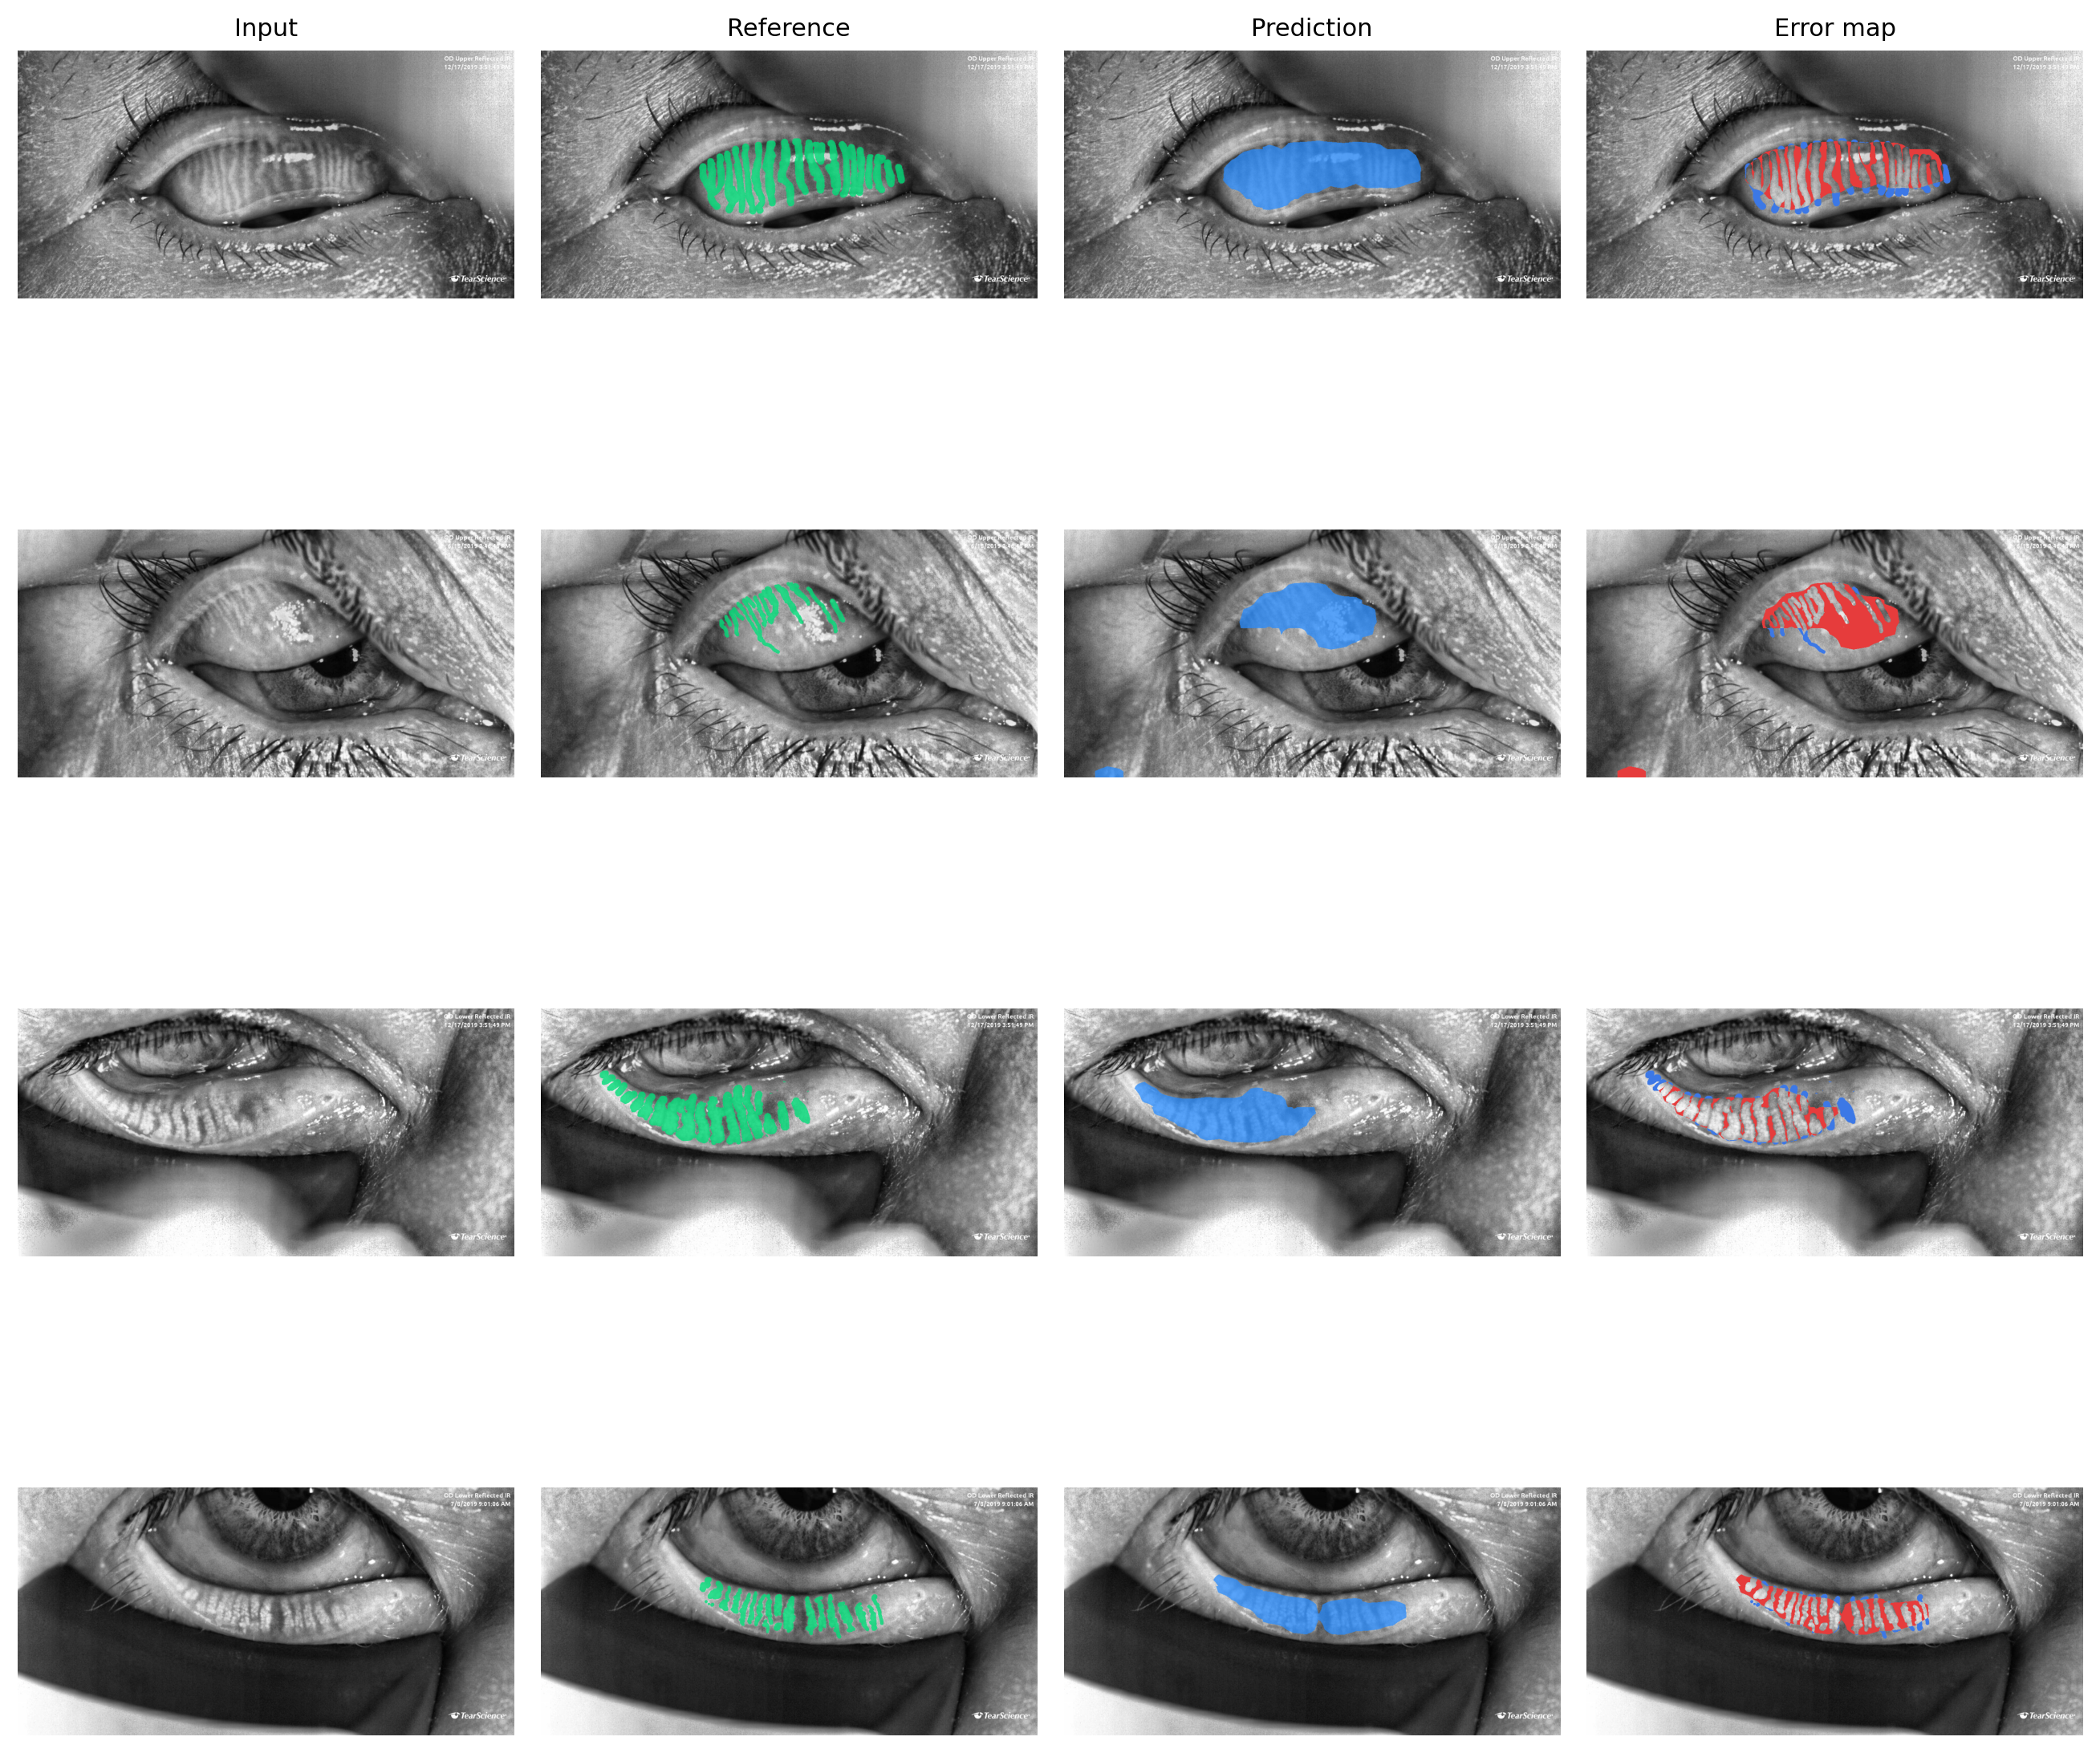
\includegraphics[width=\linewidth]{figures/qualitative.png}
\caption{Qualitative results: input, expert reference, model prediction, and error map (red = false positive, blue = false negative). Rows are selected across upper/lower eyelids; the error map shows breaks, merges, and eyelid leakage, and does not replace metrics.}
\label{fig:qualitative}
\end{figure}


\subsection{Legacy Weights as an Engineering Anchor}

The legacy UNet weights came from a script that shuffled all \nTotal{} cases with no holdout, so their ``test'' metrics may be train-self and the official 200 test list may be inside their training data. We use them only as an engineering regression anchor: Dice \legacyUNetSelfDice, IoU \legacyUNetSelfIoU, clDice \legacyUNetSelfClDice. These values \textbf{must not} enter any independent-test table and must not be compared with the models here.

\subsection{Discussion}

Taken together, the argument is not that one backbone wins everywhere, but three things: first, patient-level splitting changes conclusions, and a public benchmark must report an assignment signature; second, tiling is an experimental variable on par with the backbone, and MTE offers a no-retraining stabiliser; third, pixel metrics and clinical grading must be reported together, because ``better segmentation'' may not mean ``better grading''. These three points are closer to clinically usable evidence than yet another backbone.
